%%%%%%%%%%%%%%%%%%%%%%%%%%%%%%%%%%%%%%%%%%%%%%%%%%%%%%%%%%%%%%%%%%%%%%%%%%%%%%%
%                         File: osa-revtex4-1.tex                             %
%                        Date: April 15, 2013                                 %
%                                                                             %
%                              BETA VERSION!                                  %
%                   JOSA A, JOSA B, Applied Optics, Optics Letters            %
%                                                                             %
%            This file requires the substyle file osajnl4-1.rtx,              %
%                   running under REVTeX 4.1 and LaTeX 2e                     %
%                                                                             %
%                   USE THE FOLLOWING REVTeX 4-1 OPTIONS:                     %
% \documentclass[osajnl,twocolumn,showpacs,superscriptaddress,10pt]{revtex4-1}%
%                    %% Use 11pt for Applied Optics                           %
%                                                                             %
%               (c) 2013 The Optical Society of America                       %
%                                                                             %
%%%%%%%%%%%%%%%%%%%%%%%%%%%%%%%%%%%%%%%%%%%%%%%%%%%%%%%%%%%%%%%%%%%%%%%%%%%%%%%

\documentclass[osajnl,twocolumn,showpacs,superscriptaddress,10pt]{revtex4-1} %% use 11pt for Applied Optics
%%\documentclass[osajnl,preprint,showpacs,superscriptaddress,12pt]{revtex4-1} %% use 12pt for preprint option
\usepackage{amsmath,amssymb,graphicx,float,minted}
\usepackage[utf8]{inputenc}
\graphicspath{ {images/} }

\begin{document}

\title{SGEMM GPU kernel performance Data Set}

\author{Ulises Jeremias Cornejo Fandos}
\affiliation{Licenciatura en Informatica - 13566/7, Facultad de Informatica, UNLP}

\author{Gaston Gustavo Rios}
\affiliation{Licenciatura en Informatica - 13591/9, Facultad de Informatica, UNLP}


\begin{abstract}
En el presente informe se dispone el análisis realizado a \textit{SGEMM GPU kernel performance Data Set} así como tambien el proceso de construcción de modelos de sistemas inteligentes entrenados con el fin de resolver un problema en forma eficiente y que se ajuste a las necesidades impuestas. Como se explica en el informe, se utilizan variadas tecnologías para la construcción y análisis de estos modelos así como tambien la evaluación de performance de los mismos. \\
\end{abstract}

\maketitle %% required

\section{Introducción}

\subsection{SGEMM GPU kernel performance Data Set}

El conjunto de datos a analizar mide el tiempo de ejecución, \textit{en milisegundos}, de un producto matriz-matriz $A * B = C$, donde las matrices tienen un tamaño de $2048 x 2048$, usando un núcleo de \textit{GPU SGEMM} parametrizable con \textit{241600} posibles combinaciones de parámetros. Para cada combinación probada, se realizan 4 corridas y sus resultados se disponen en las ultimas 4 columnas. \\

Hay 14 parámetros, los primeros 10 son ordinales y solo pueden tomar hasta 4 potencias diferentes de dos valores, y las 4 últimas variables son binarias. De las 1327104 combinaciones de parámetros totales, solo 241600 son factibles \textit{(debido a varias restricciones del kernel)}. Este conjunto de datos contiene los resultados de todas estas combinaciones posibles. \\

El experimento se ejecutó en una estación de trabajo de escritorio que ejecuta Ubuntu 16.04 Linux con un Intel Core i5 (3.5GHz), 16GB de RAM y una NVidia Geforce GTX 680 4GB GF580 GTX-1.5GB GPU. Se utiliza el kernel \textit{gemm\_fast} de la biblioteca de sintonización de kernel automática de OpenCL 'CLTune'. \\

\subsubsection{}{Información de los atributos}

\begin{itemize}
    \item \textbf{Variables independientes}

    \begin{itemize}
        \item \textit{1-2. $M_{wg}$, $N_{wg}$:} bloque 2D por matriz a nivel de grupo de trabajo. Toma valores enteros del conjunto $\{16, 32, 64, 128\}$.
        \item \textit{3. $K_{wg}$:} dimesión interna del bloque 2D a nivel de grupo de trabajo. Toma valores enteros del conjunto $\{16, 32\}$.
        \item \textit{4-5. $M_{dim}C$, $N_{dim}C$:} tamaño del grupo de trabajo local. Toma valores enteros del conjunto $\{8, 16, 32\}$.
        \item \textit{6-7. $M_{dim}A$, $N_{dim}B$:} forma de la memoria local. Toma valores enteros del conjunto $\{8, 16, 32\}$.
        \item \textit{8. $K_{wi}$:} factor de desenrollado del bucle del kernel. Toma valores enteros del conjunto $\{2, 8\}$.
        \item \textit{9-10. $V_{wm}$, $V_{wn}$:} anchos de vectores por matriz para cargar y almacenar. Toma valores enteros del conjunto $\{1, 2, 4, 8\}$.
        \item \textit{11-12. $M_{stride}$, $N_{stride}$:} stride habilitado para acceder a la memoria off-chip en un único hilo. Variable binaria.
        \item \textit{13-14. $S_{A}$, $S_{B}$:} Almacenamiento en caché manual por matriz del mosaico del grupo de trabajo 2D. Variable binaria.
    \end{itemize}

    \begin{itemize}
        \item \textit{15-18. $Run_1$, $Run_2$, $Run_3$, $Run_4$:} tiempos de rendimiento en milisegundos para 4 ejecuciones independientes con los mismos parámetros. Toman valores reales del intervalo $[13.25, 3397.08]$.
    \end{itemize}
\end{itemize}

\subsection{Conjunto de datos a analizar}

Para decidir las tecnologías y conjunto de datos a utilizar se evalúan distintas posibilidades intentando optar por la que mejor se adapte a las necesidades y dominio del problema. \\

Como se muestra en la sub-sección anterior, el conjunto de datos planteado dispone de una gran cantidad de ejemplos \textit{(241600 combinaciones de parámetros)}. Para realizar el análisis sobre este conjunto de datos, se busca utilizar un software el cual permite el análisis de hasta 10000 ejemplos, por lo que se reduce el tamaño del espacio muestral a utilizar buscando no perder información relevante para el dominio del problema. \\

Para esto se decide que sería conveniente evaluar cuáles de esos parámetros son más relevantes y, a su vez, cuáles de los valores tomados por cada uno generan cambios reales en los tiempos de ejecución resultante. Para esto se limita esta evaluación a aquellos parámetros cuyos posibles valores pertenezcan a un conjunto de cardinalidad mayor que dos, dado que así presentan más configuraciones posibles. \\

Se toman los parámetros $M_{wg}$ y $N_wg$ solo las filas que tienen valores pertenecientes a $\{64, 128\}$, quedando así la mitad de ejemplos. Esta cantidad se puede reducir más fijando alguno de los parámetros, lo cual sería muy conveniente. Luego, se observa que en dos de los datos categóricos, la configuración más eficiente es $(S_{A}, S_{B}) = (1, 1)$. De esto surge la duda de si podrían quitarse los casos en los que uno de ellos, o ambos, sean “no”. Se considera que con esto podría reducirse lo suficiente para poder así procesar los datos. Y finalmente tenemos que buscar cómo podemos dividirlo en dos data sets. \\

Aplicando dichas reducciones se ve que con el conjunto de datos resultante se pierde mucha información potencialmente valiosa. Es por esto que se decide evaluar nuevas posibilidades llegando así a la opción utilizada. \\

Se opta por analizar y construir modelos de sistemas inteligentes evaluando la totalidad de los datos utilizando nuevas tecnologías de las cuales se detalla más en la siguientes subsecciones. \\

El conjunto de datos permanece intacto comparado con el original a diferencia de las columnas de tiempo de ejecución que se descartan luego de generar un único atributo el cual sea igual a la media de los 4 anteriores. \\

\section{Marco Teórico}

En esta sección se introduce brevemente conceptos básicos necesarios para abordar los contenidos de las siguientes secciones del informe con mayores referencias y capacidad de entendimiento. \\

\subsection{Representaciones Gráficas}

\subsubsection{Diagrama de dispersión}

Un \textbf{diagrama de dispersión} es un tipo de diagrama matemático que utiliza las coordenadas cartesianas para mostrar los valores de dos variables para un conjunto de datos. \\

Se emplea cuando una variable está bajo el control del experimentador. Si existe un parámetro que se incrementa o disminuye de forma sistemática por el experimentador, se le denomina parámetro de control o variable independiente y habitualmente se representa a lo largo del eje horizontal (eje de las abscisas). La variable medida o dependiente usualmente se representa a lo largo del eje vertical (eje de las ordenadas). Si no existe una variable dependiente, cualquier variable se puede representar en cada eje y el diagrama de dispersión mostrará el grado de correlación (no causalidad) entre las dos variables. \\

Un diagrama de dispersión puede sugerir varios tipos de correlaciones entre las variables con un intervalo de confianza determinado. La correlación puede ser positiva (aumento), negativa (descenso), o nula (las variables no están correlacionadas).

\subsubsection{Diagrama de Caja}

Un \textbf{diagrama de caja}, también conocido como \textit{diagrama de caja y bigotes}, es un gráfico que está basado en cuartiles y mediante el cual se visualiza la distribución de un conjunto de datos. Está compuesto por un rectángulo (la caja) y dos brazos (los bigotes). \\

Es un gráfico que suministra información sobre los valores mínimo y máximo, los cuartiles Q1, Q2 o mediana y Q3, y sobre la existencia de valores atípicos y la simetría de la distribución. Primero es necesario encontrar la mediana para luego encontrar los 2 cuartiles restantes. \\

Un diagrama de cajas proporcionan una visión general de la simetría de la distribución de los datos; si la mediana no está en el centro del rectángulo, la distribución no es simétrica. Son útiles para ver la presencia de valores atípicos también llamados outliers. Pertenece a las herramientas de las estadística descriptiva. Permite ver como es la dispersión de los puntos con la mediana, los percentiles 25 y 75 y los valores máximos y mínimos. Ponen en una sola dimensión los datos de un histograma, facilitando así el análisis de la información al detectar que el 50\% de la población está en los límites de la caja.

\subsubsection{Histograma}

En estadística, un \textbf{histograma} es una representación gráfica de una variable en forma de barras, donde la superficie de cada barra es proporcional a la frecuencia de los valores representados. Sirven para obtener una "primera vista" general, o panorama, de la distribución de la población, o de la muestra, respecto a una característica, cuantitativa y continua (como la longitud o el peso). De esta manera ofrece una visión de grupo permitiendo observar una preferencia, o tendencia, por parte de la muestra o población por ubicarse hacia una determinada región de valores dentro del espectro de valores posibles (sean infinitos o no) que pueda adquirir la característica.

\subsubsection{Diagramas de Barras}

Un \textbf{diagrama de barras} es una forma de representar gráficamente un conjunto de datos o valores, y está conformado por barras rectangulares de longitudes proporcionales a los valores representados. Los gráficos de barras son usados para comparar dos o más valores. Las barras pueden orientarse horizontal o verticalmente.

\subsection{Clustering}

Un algoritmo de agrupamiento (en inglés, clustering) es un procedimiento de agrupación de una serie de vectores de acuerdo con un criterio. Esos criterios son por lo general distancia o similitud. La cercanía se define en términos de una determinada función de distancia, como la euclídea, aunque existen otras más robustas o que permiten extenderla a variables discretas. La medida más utilizada para medir la similitud entre los casos es la matriz de correlación entre los nxn casos. Sin embargo, también existen muchos algoritmos que se basan en la maximización de una propiedad estadística llamada verosimilitud. \\

En el contexto de la Mineria de Datos se lo considera una técnica de aprendizaje no supervisado puesto que busca encontrar relaciones entre variables descriptivas pero no la que guardan con respecto a una variable objetivo. \\

\subsubsection{K-Means}

\textbf{K-means} es un método de agrupamiento, que tiene como objetivo la partición de un conjunto de n observaciones en k grupos en el que cada observación pertenece al grupo cuyo valor medio es más cercano. \\

En la figura \ref{figure:clustering_example} se muestra un ejemplo de aplicación del algoritmo k-means para realizar un agrupamiento de los datos.

\begin{figure}[H]
    \centering
    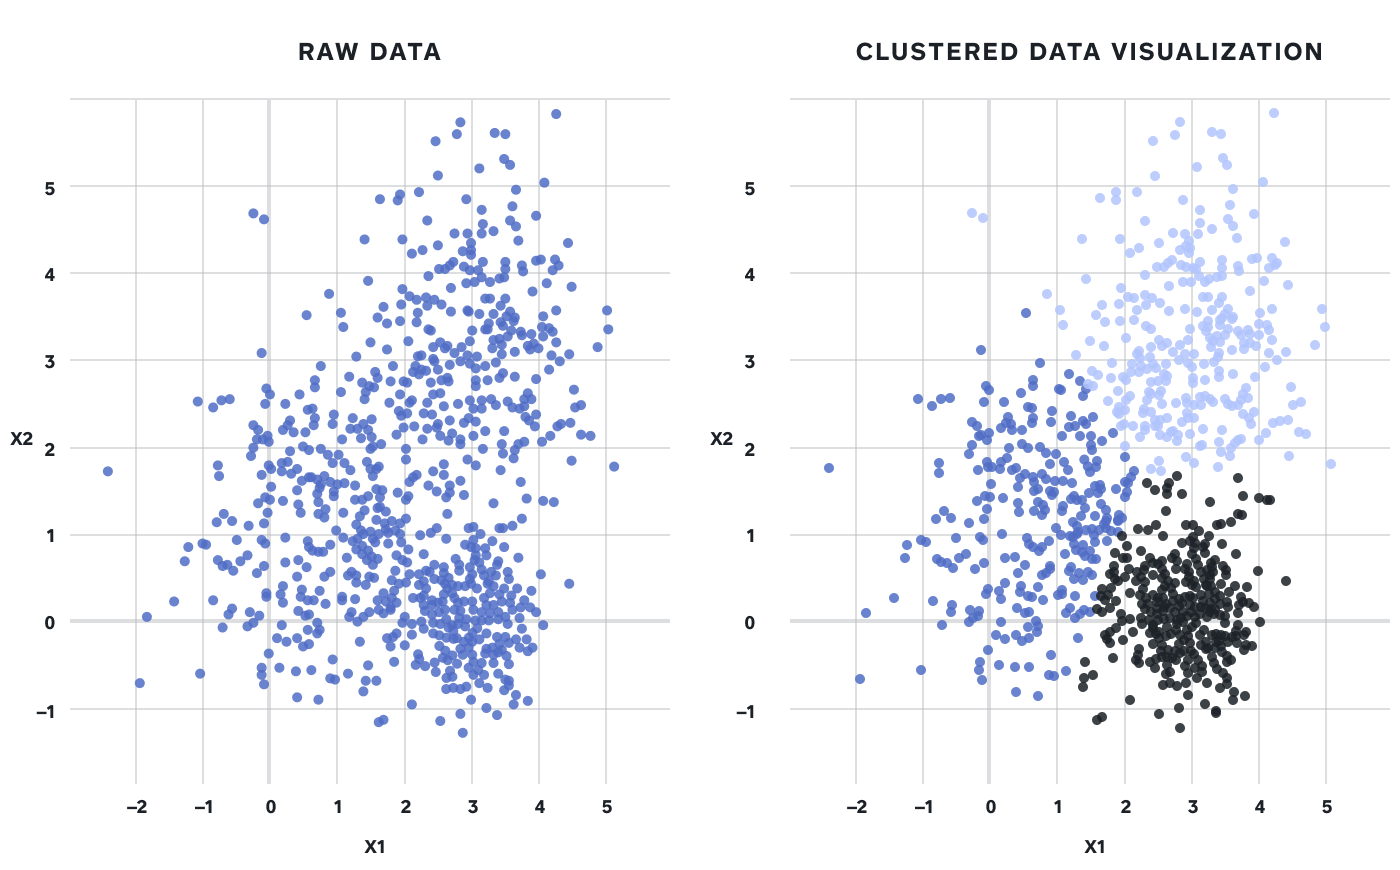
\includegraphics[width=0.4\textwidth]{theory/clustering}
    \caption{Ejemplo de aplicación del algoritmo k-means para realizar un agrupamiento de los datos.}
    \label{figure:clustering_example}
\end{figure}

\subsection{Redes Neuronales}

Las \textbf{redes neuronales} son un modelo computacional basado en un gran conjunto de unidades neuronales simples, \textbf{neuronas artificiales}, de forma aproximadamente análoga al comportamiento observado en los axones de las neuronas en los cerebros biológicos. \\

Cada unidad neuronal está conectada con muchas otras y los enlaces entre ellas pueden incrementar o inhibir el estado de activación de las neuronas adyacentes. Cada unidad neuronal, de forma individual, opera empleando funciones de suma. Puede existir una función limitadora o umbral en cada conexión y en la propia unidad, de tal modo que la señal debe sobrepasar un límite antes de propagarse a otra neurona. \\

Estos sistemas aprenden y se forman a sí mismos, en lugar de ser programados de forma explícita, y sobresalen en áreas donde la detección de soluciones o características es difícil de expresar con la programación convencional.

\subsubsection{Perceptron}

En el campo de las Redes Neuronales, el \textbf{perceptrón}, se refiere a la neurona artificial o unidad básica de inferencia en forma de discriminador lineal, a partir del cual se desarrolla un algoritmo capaz de generar un criterio para seleccionar un sub-grupo a partir de un grupo de componentes más grande. \\

En la figura (\ref{figure:perceptron_example}) se muestra la arquitectura que determina el comportamiento de un perceptron.

\begin{figure}[H]
    \centering
    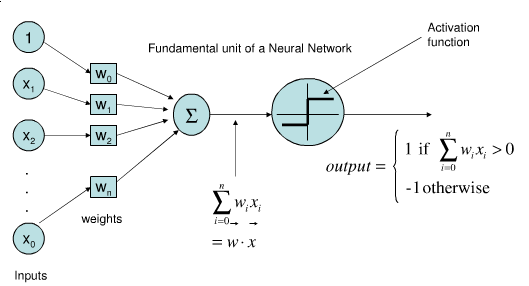
\includegraphics[width=0.4\textwidth]{theory/perceptron}
    \caption{Arquitectura de un perceptron.}
    \label{figure:perceptron_example}
\end{figure}

La limitación de este algoritmo es que si dibujamos en un gráfico estos elementos, se deben poder separar con un hiperplano únicamente los elementos "deseados" discriminándolos (ó \textit{separándolos}) de los \textit{"no deseados"} como se muestra en la figura (\ref{figure:linear_example}).

\begin{figure}[H]
    \centering
    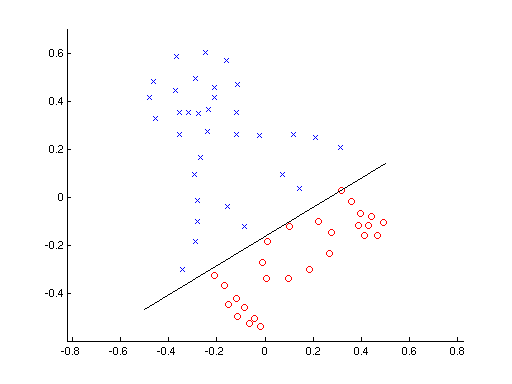
\includegraphics[width=0.4\textwidth]{theory/linear}
    \caption{Ejemplo de función linear discriminante.}
    \label{figure:linear_example}
\end{figure}

El perceptrón puede utilizarse con otros tipos de perceptrones o de neurona artificial, para formar una red neuronal artificial más compleja.

\subsubsection{Multiperceptrón}

El \textbf{perceptrón multicapa}, \textit{multi-perceptrón}, es una red neuronal artificial formada por múltiples capas, de tal manera que tiene capacidad para resolver problemas que no son linealmente separables que, como se explica en la subsección anterior, es la principal limitación del \textit{perceptrón}. El perceptrón multicapa puede estar totalmente o localmente conectado. En el primer caso cada salida de una neurona de la capa \textit{"i"} es entrada de todas las neuronas de la capa \textit{"i+1"}, mientras que en el segundo cada neurona de la capa \textit{"i"} es entrada de una serie de neuronas (región) de la capa \textit{"i+1"}. \\

Se muestra en la figura (\ref{figure:multiperceptron_example}) un ejemplo de la arquitectura de un perceptron multicapa.

\begin{figure}[H]
    \centering
    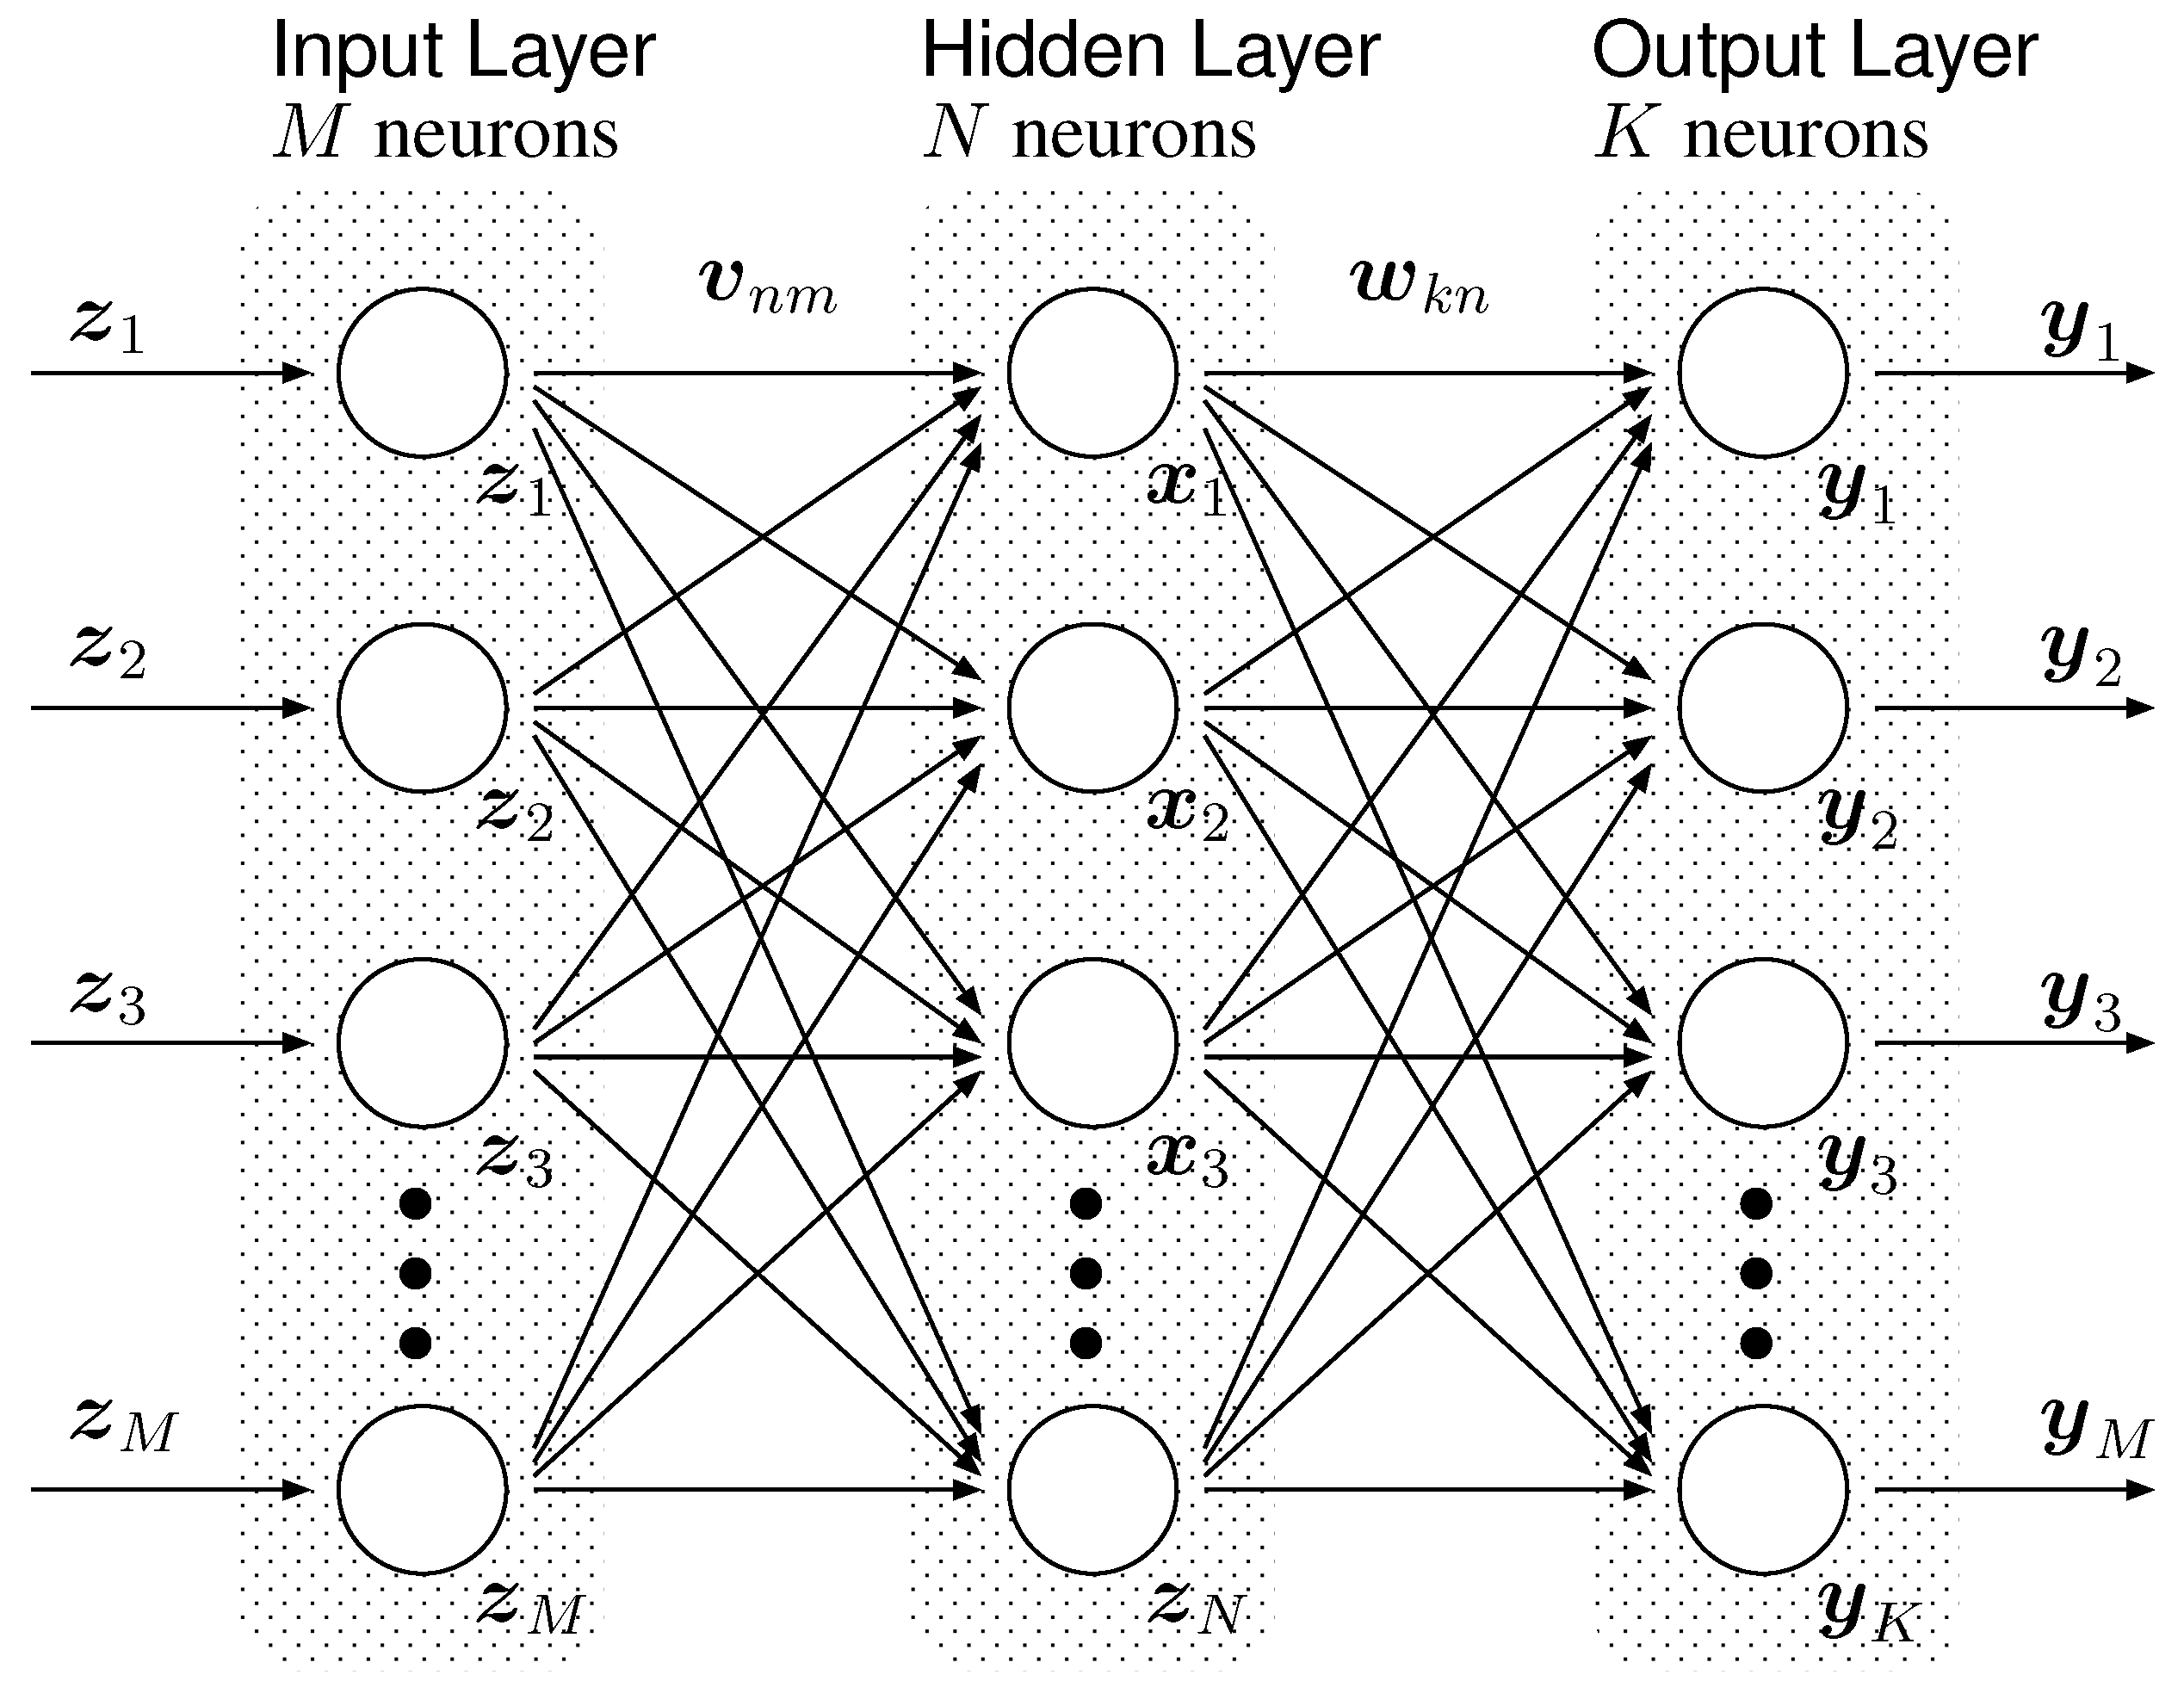
\includegraphics[width=0.4\textwidth]{theory/multiperceptron}
    \caption{Ejemplo básico de un multiperceptron.}
    \label{figure:multiperceptron_example}
\end{figure}

\section{Análisis de datos}

Para el análisis de los datos se evalúan distintas gráficas de los mismos, como histogramas de los datos nominales y gráficas de dispersión para aquellos datos de tipo numérico, además de ciertas métricas que permiten conocer la correlación entre cada uno de ellos. De este modo se permite observar relaciones entre los distintos atributos del conjunto de datos así como también la relación entre estos mismos y la etiqueta, o \textit{label}.

\begin{flushright}
\textit{\footnotesize Se dispone de las gráficas correspondientes a los atributos en la sección \ref{apendix:images:attr} del apéndice.}
\end{flushright}

Mencionando alguna de las gráficas que se puenden observar en el apendice tenemos la figura (\ref{figure:run_hist_1}). En la misma se puede observar una asimetría en la distribución de los valores, notando que existe mayor número de instancias en las que el tiempo de ejecución tiende al valor mínimo.

\begin{figure}[H]
    \centering
    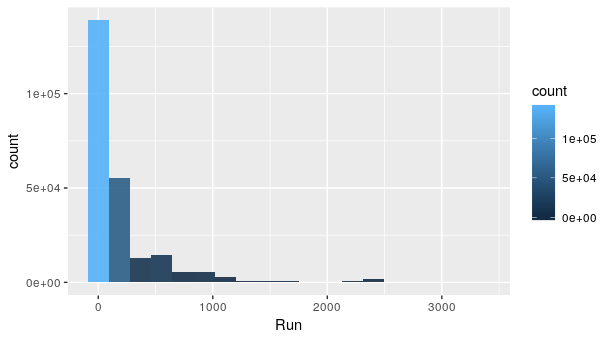
\includegraphics[width=0.45\textwidth]{plots/run_hist}
    \caption{Histograma del atributo Run.}
    \label{figure:run_hist_1}
\end{figure}

\begin{flushright}
\textit{\footnotesize Se dispone de una explicación del código utilizado para generar los gráficos en la sección \ref{apendix:scripts} del apéndice.}
\end{flushright}

\section{Hipótesis y Objetivos}

Analizando las gráficas se cree que existen valores que pueden ser indistintos al momento de definir la mejor configuración de parámetros. Por lo tanto se tiene como objetivo determinar cuales son, así como tambien buscar la forma de construir una red neuronal capaz de predecir el tiempo de ejecución de la función para una configuración dada. \\

\section{Método Experimental} \label{section:experimental_method}

En esta sección se detalla todo lo referido al estudio y la creación de los distintos modelos de sistemas inteligentes utilizados para el estudio del conjunto de datos elegido. \\

Para el análisis de este dataset se utilizan dos modelos de sistemas inteligentes detallados a continuación. \\

\section{Clustering}

\subsection{K-Means}

Para la construcción de este modelo se utiliza el algoritmo K-means evaluando las distancias con distancia euclidea. Se evalúa la calidad del modelo resultante utilizando el índice de Silhouette notando que se obtienen mejores resultandos cuando el número de clusters $k$ es igual a 2, obteniendo finalmente un índice de Silhouette igual a 0.824. Cabe destacar que el indice obtenido se calcula utilizando $1000$ ejemplos dado que resulta imposible utilizar la totalidad de los datos debido al consumo exesivo de memoria. Una comparativa entre la cantidad de clusters y el indice de Silhouette obtenido se puede observar en la tabla (\ref{table:clusters_silhouette}). \\

\begin{table}[h!]
    \centering
    \begin{tabular}{ccccccc}
        centroides & tiempo & silhouette \\
        \hline
        2 & 1.60s	& 0.824 \\
        3 & 1.42s	& 0.749 \\
        4 & 3.19s	& 0.587 \\
        5 & 3.26s	& 0.512 \\
        6 & 2.43s	& 0.503 \\
        7 & 3.01s	& 0.538 \\
        8 & 3.33s	& 0.380 \\
        9 & 3.43s	& 0.396 \\
        \hline
    \end{tabular}
    \caption{Comparativa entre la cantidad de clusters y el indice de Silhouette obtenido}
    \label{table:clusters_silhouette}
\end{table}

Como resultado se obtienen dos agrupamientos, \textit{cluster\_0} y \textit{cluster\_1}. Se pueden ver los datos del agrupamiento en la tabla (\ref{table:k_means}).

\begin{table}[h!]
    \centering
    \begin{tabular}{|ccc|ccc|}
        \hline
        cluster & atributo & centroide & cluster & atributo & centroide \\
        \hline
        0	& MWG & 77.454 & 1 &	MWG & 116.948 \\
        0	& NWG & 77.428 & 1 &	NWG & 117.277 \\
        0	& KWG & 25.436 & 1 &	KWG & 26.465 \\
        0	& MDIMC & 14.294 & 1 &	MDIMC & 9.517 \\
        0	& NDIMC & 14.316 & 1 &	NDIMC & 9.241 \\
        0	& MDIMA & 17.385 & 1 &	MDIMA & 17.201 \\
        0	& NDIMB & 17.380 & 1 &	NDIMB & 17.265 \\
        0	& KWI & 4.955 & 1 &	KWI & 5.556 \\
        0	& VWM & 2.382 & 1 &	VWM & 3.266 \\
        0	& VWN & 2.387 & 1 &	VWN & 3.211 \\
        0	& STRM & 0.500 & 1 &	STRM & 0.502 \\
        0	& STRN & 0.500 & 1 &	STRN & 0.505 \\
        0	& SA & 0.482 & 1 &	SA & 0.723 \\
        0	& SB & 0.482 & 1 &	SB & 0.720 \\
        0	& Run & 132.668 & 1 &	Run & 1265.095 \\
        \hline
    \end{tabular}
    \caption{Resultados del clustering generado con k\_means}
    \label{table:k_means}
\end{table}

\subsection{Redes Neuronales}

Para crear un modelo de redes neuronales que se adapte a las necesidades planteadas anteriormente se opta por la utilización de librerías las cuales permitan un desarrollo cómodo utilizando el lenguaje de programación Python. Es por esto que se decide utilizar \textit{SKLearn} para un preprocesamiento extra de los datos como puede ser la normalización de los mismos utilizando normalización Z, \textit{Pandas} para lectura y escritura de datos en formato csv y \textit{TensorFlow} como principal librería de computación de numérica para la creación y entrenamiento de modelos de redes neuronales. \\

\begin{flushright}
\textit{\footnotesize Se dispone de una explicación del código y los modelos generados en la sección \ref{apendix:scripts} del apéndice.}
\end{flushright}

En resumen el modelo se construye a partir de 3 capas ocultas con una cantidad maxima de 256 neuronas y las siempre presentes capas de input y output siendo entonces un total de 5 capas. Se utiliza ReLu como función de actualización, una capa de transposición en el output, el error cuadrático medio como función de costo y AdamOptimicer como optimizador de la función. Se realizan 20 epochs y 256 batchs. Cuanta mayor cantidad de batchs, mas rapido será el entrenamiento pero se consiguen peores resultados. Cabe descatacar que la cantidad de batchs se ve limitada por la cantidad de memoria disponible. \\

Como se observa en la explicación mencionada el modelo generado resulta en un error cuadrático medio de 0.0010947415 para los datos de entrenamiento y 0.0012081241 para los datos de test. Es por esto que se puede afirmar que el modelo generado tiene un gran nivel de generalización y presición en la estimación del tiempo de ejecución. \\

A su vez, el modelo generado permite predecir la mejor configuración de parámetros con el mejor tiempo de ejecución posible siendo este cuando $M_{wg} = 128$, $N_{wg} = 128$,  $K_{wg} = 32$,  $M_{dim}C = 32$, $N_{dim}C = 32$, $M_{dim}A = 32$, $ N_{dim}B = 32$, $K_{wi} = 2$, $V_{wm} = 4$, $V_{wn} = 4$, $M_{stread} = 1$, $N_{stread} = 1$, $S_A = 1$ y $S_B = 1$. \\

\section{Análisis de Resultados} \label{section:results_analysis}

En esta sección se analizan los resultados obtenidos en el método experimental con el fin de introducir algunos aspectos escenciales para discución de los mismos y conclusiones a tomar. \\

A partir del agrupamiento generado se puede determinar aquellas configuraciones relevantes para determinar el tiempo de ejecución de la función sabiendo entonces que es indistintos el valor de los parámetros KWG, MDIMA, MDIMB, KWI, STRM y STRN. Por otro lado podemos observar que las configuraciones pertenecientes al $cluster\_0$ serán las más eficientes. \\

Por otro lado, se sabe que es posible encontrar un modelo de redes neuronales el cual, dada una configuración de parámetros, prediga el tiempo de ejecución correspondiente. Particularmente el mismo encuentra así la configuración más eficiente la cual se puede observar en la sección anterior. \\

\section{Discusión y Conclusiones}

A lo largo del método experimental descripto en la sección \ref{section:experimental_method} se obtienen dos modelos con una gran precisión, lo cual nos permite concluir que es posible estudiar este problema e incluso llegar a predecir de forma eficiente el tiempo de ejecución de la función a partir de una configuración de parámetros dada. \\

Al mismo tiempo se determina que el existe un subconjunto de parámetros que afectan en mayor medida al tiempo de ejecución así como tambien otro subconjunto que resulta indistinto al momento de determinar una configuración eficiente. \\

\begin{thebibliography}{99}
%% Do not include separate BibTeX files; if BibTeX is used,
%% paste the output (contents of .bbl file) here.

\bibitem{project} \url{https://github.com/ulises-jeremias/midusi}
\bibitem{r-project} \url{https://www.r-project.org}.
\bibitem{python 3} \url{https://www.python.org/doc}.
\bibitem{numpy} \url{www.numpy.org}
\bibitem{sk-learn} \url{www.scikit-learn.org}
\bibitem{tensorflow} \url{www.tensorflow.org}
\bibitem{ml_postgrado} Aceleración de algoritmos de Machine Learning desde un punto de vista Arquitectónico, Curso de Postgrado, Facultad de Informática, UNLP.
\bibitem{tensorflow_example} https://medium.com/mlreview/a-simple-deep-learning-model-for-stock-price-prediction-using-tensorflow-30505541d877

\end{thebibliography}

\clearpage

\onecolumngrid

\section{Apéndice}

\subsection{Imágenes}

\subsubsection{Gráficos de los atributos} \label{apendix:images:attr}

\twocolumngrid

\begin{figure}[H]
    \centering
    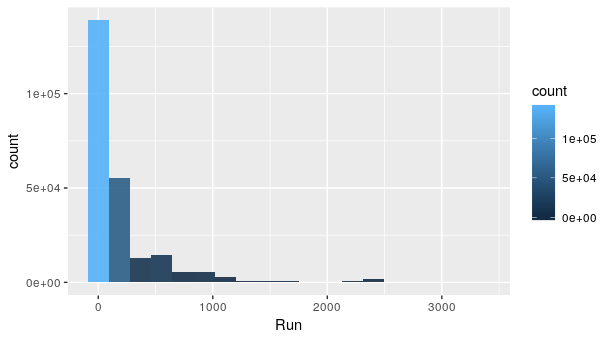
\includegraphics[width=0.45\textwidth]{plots/run_hist}
    \caption{Histograma del atributo Run.}
    \label{figure:run_hist}
\end{figure}

\begin{figure}[H]
    \centering
    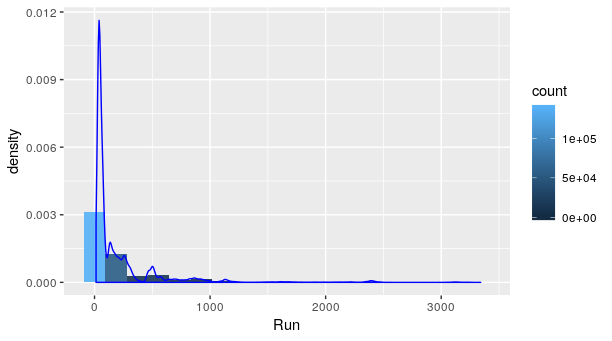
\includegraphics[width=0.45\textwidth]{plots/run_density}
    \caption{Histograma y gráfica de densidad del atributo Run.}
    \label{figure:run_density}
\end{figure}

\begin{figure}[H]
    \centering
    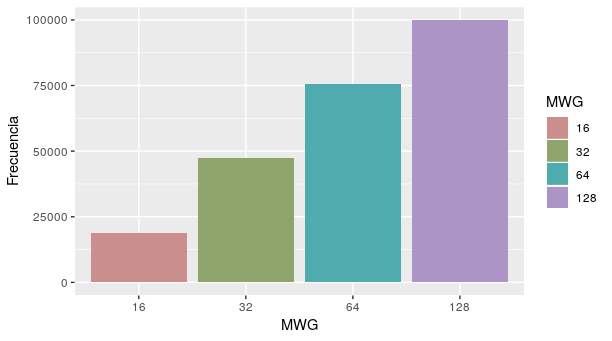
\includegraphics[width=0.45\textwidth]{plots/mwg_bar}
    \caption{Gráfico de barras del atributo $M_{wg}$.}
    \label{figure:mwg_bar}
\end{figure}

\begin{figure}[H]
    \centering
    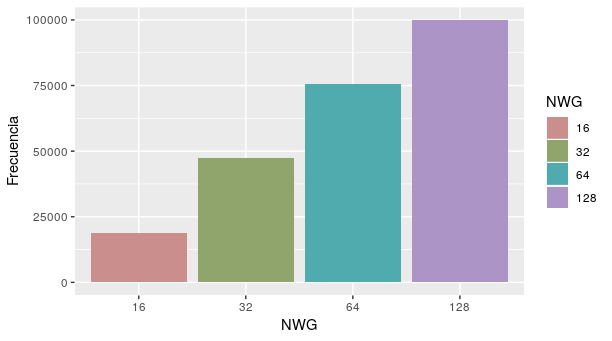
\includegraphics[width=0.45\textwidth]{plots/nwg_bar}
    \caption{Gráfico de barras del atributo $N_{wg}$.}
    \label{figure:nwg_bar}
\end{figure}

\begin{figure}[H]
    \centering
    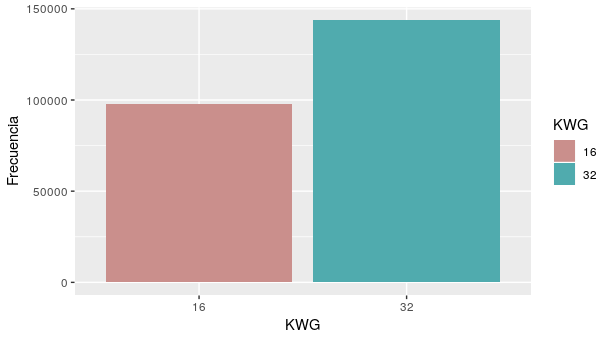
\includegraphics[width=0.45\textwidth]{plots/kwg_bar}
    \caption{Gráfico de barras del atributo $K_{wg}$.}
    \label{figure:kwg_bar}
\end{figure}

\begin{figure}[H]
    \centering
    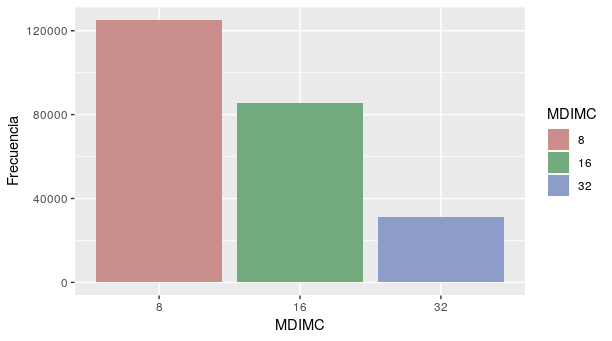
\includegraphics[width=0.45\textwidth]{plots/mdimc_bar}
    \caption{Gráfico de barras del atributo $M_{dim}C$.}
    \label{figure:MDIMC_bar}
\end{figure}

\begin{figure}[H]
    \centering
    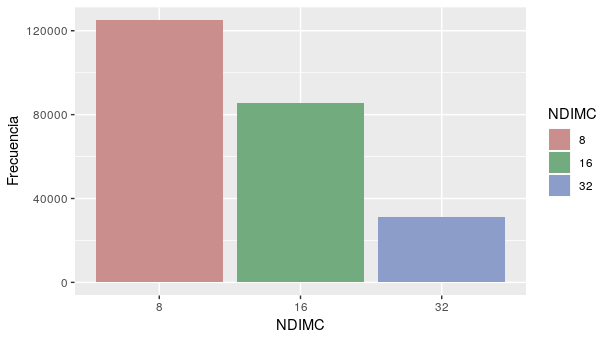
\includegraphics[width=0.45\textwidth]{plots/ndimc_bar}
    \caption{Gráfico de barras del atributo $N_{dim}C$.}
    \label{figure:ndimc_bar}
\end{figure}

\begin{figure}[H]
    \centering
    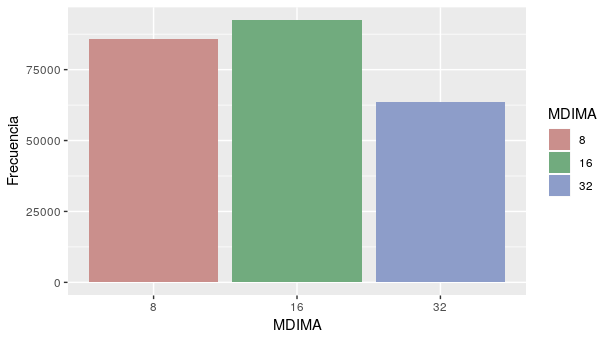
\includegraphics[width=0.45\textwidth]{plots/mdima_bar}
    \caption{Gráfico de barras del atributo $M_{dim}A$.}
    \label{figure:mdima_bar}
\end{figure}

\begin{figure}[H]
    \centering
    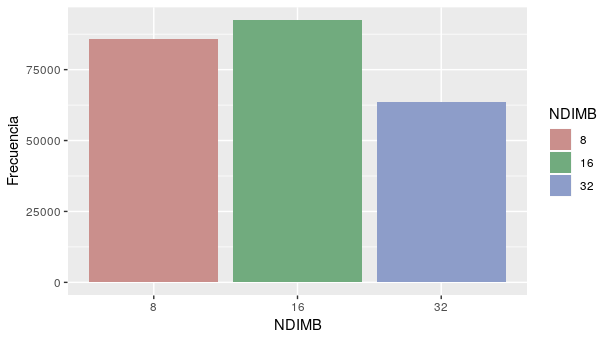
\includegraphics[width=0.45\textwidth]{plots/ndimb_bar}
    \caption{Gráfico de barras del atributo $N_{dim}B$.}
    \label{figure:ndimb_bar}
\end{figure}

\begin{figure}[H]
    \centering
    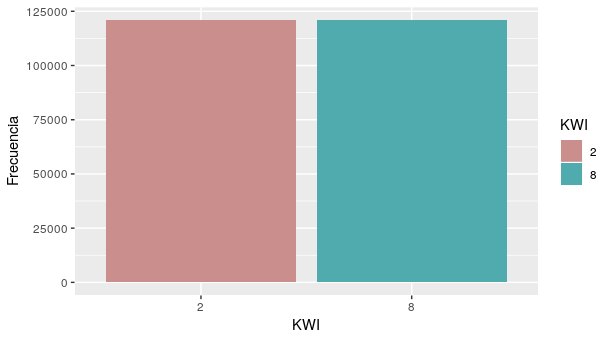
\includegraphics[width=0.45\textwidth]{plots/kwi_bar}
    \caption{Gráfico de barras del atributo $K_{wi}$.}
    \label{figure:kwi_bar}
\end{figure}

\begin{figure}[H]
    \centering
    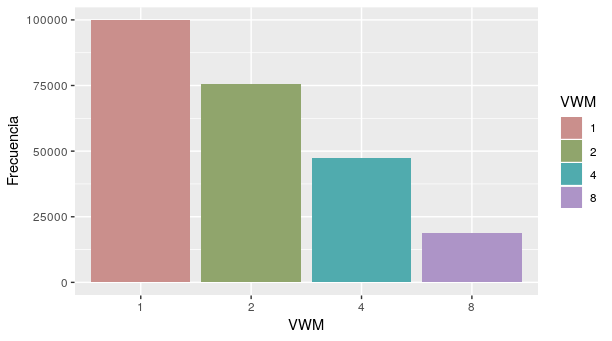
\includegraphics[width=0.45\textwidth]{plots/vwm_bar}
    \caption{Gráfico de barras del atributo $V_{wm}$.}
    \label{figure:vwm_bar}
\end{figure}

\begin{figure}[H]
    \centering
    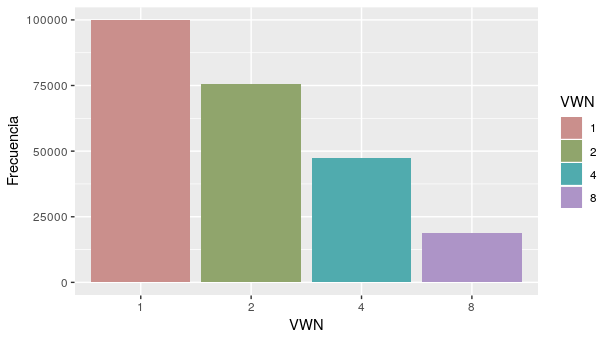
\includegraphics[width=0.45\textwidth]{plots/vwn_bar}
    \caption{Gráfico de barras del atributo $V_{wn}$.}
    \label{figure:vwn_bar}
\end{figure}

\begin{figure}[H]
    \centering
    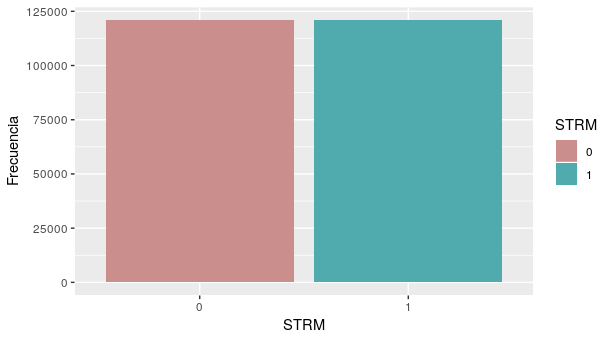
\includegraphics[width=0.45\textwidth]{plots/strm_bar}
    \caption{Gráfico de barras del atributo $M_{stride}$.}
    \label{figure:strm_bar}
\end{figure}

\begin{figure}[H]
    \centering
    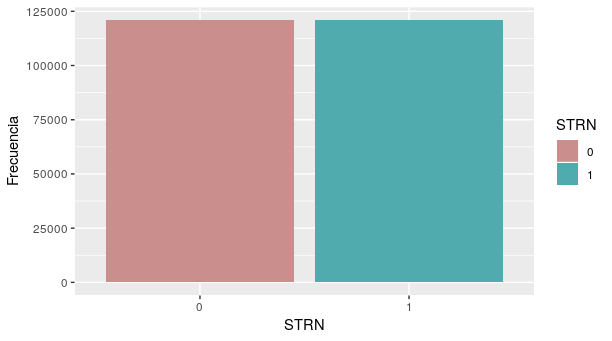
\includegraphics[width=0.45\textwidth]{plots/strn_bar}
    \caption{Gráfico de barras del atributo $N_{stride}$.}
    \label{figure:strn_bar}
\end{figure}

\onecolumngrid

\subsection{Scripts y Modelos} \label{apendix:scripts}

Todo el material presentado en esta sección así como tambien los modelos entrenados y scripts utilizados, pero no referenciados en el presente documento, pueden encontrarse en el siguiente repositorio de github: \url{https://github.com/ulises-jeremias/midusi}.

\subsubsection{Gráficos y preprocesamiento de datos}

Se utiliza R para el filtrado y graficado de los datos. Para esto se dispone de dos scrips. \\

El primero permite la creación del conjunto de datos a analizar. Puede nortarse que la linea de código comentada corresponde al filtrado de datos a utilizar en caso de utilizar RapidMiner. \\

\begin{minted}[mathescape,
               linenos,
               numbersep=5pt,
               gobble=2,
               frame=lines,
               framesep=2mm]{r}
  #!/usr/bin/env Rscript

  setwd("midusi/sgemm_product")

  originalCsvData <- read.csv(file = "data/sgemm_product.csv", head = TRUE, sep = ",")

  runColnames <- c("Run1..ms.", "Run2..ms.", "Run3..ms.", "Run4..ms.")

  cat("CSV Data type: ", class(originalCsvData), "\n")
  cat("Number of Instances: ", nrow(originalCsvData), "\n")
  cat("Number of Attributes: ", length(originalCsvData), "\n")
  cat("Attributes Name: ", colnames(originalCsvData), "\n\n\n")

  "originalCsvData <- subset(
    originalCsvData,
    MWG == NWG & (MWG == 64 | MWG == 128) &
    (SA == 1 & SB == 1)
  )"

  originalCsvData$Run <- rowMeans(originalCsvData[, runColnames], na.rm = TRUE)
  originalCsvData <- originalCsvData[, !(colnames(originalCsvData) %in% runColnames)]

  cat("Number of Instances: ", nrow(originalCsvData), "\n")
  cat("Number of Attributes: ", length(originalCsvData), "\n")
  cat("Attributes Name: ", colnames(originalCsvData), "\n")

  write.csv(originalCsvData, "filtered_sgemm_product.csv", row.names = FALSE)

  segmmProductData <- read.csv(file = "data/filtered_sgemm_product.csv", head = TRUE,
    sep = ",")

  View(segmmProductData)
\end{minted}

Luego, se genera un script capaz de graficar cada uno de los atributos utilizando gráficos de baras e histogramas. \\

Para esto, primero incluimos las dependencias y recuperamos los datos del csv de datos filtrados. Para hacer los ploteos se utiliza la librería ggplot2. \\

\begin{minted}[mathescape,
               linenos,
               numbersep=5pt,
               gobble=2,
               frame=lines,
               framesep=2mm]{r}
  #!/usr/bin/env Rscript

  library(ggplot2)

  setwd("midusi/sgemm_product")

  segmmProductData <- read.csv(file = "data/filtered_sgemm_product.csv", head = TRUE,
    sep = ",")

  View(segmmProductData)

  attach(segmmProductData)
\end{minted}

Luego, podemos graficar el histograma del atributo Run de la siguiente forma:

\begin{minted}[mathescape,
               linenos,
               numbersep=5pt,
               gobble=2,
               frame=lines,
               framesep=2mm]{r}
  # Histogram for Run column

  colmax <- max(Run, na.rm = TRUE)
  colmin <- min(Run, na.rm = TRUE)
  binwidth <- (colmax - colmin)/18

  ggplot(data = segmmProductData, aes(x = Run)) + geom_histogram(binwidth = binwidth,
    aes(fill = ..count..), alpha = 0.9) + labs(x = "Run", y = "Cantidad", fill = "Run")
\end{minted}

Y podemos obtener el gráfico de barras del atributo $M_{wg}$ de la siguiente forma:

\begin{minted}[mathescape,
               linenos,
               numbersep=5pt,
               gobble=2,
               frame=lines,
               framesep=2mm]{r}
  ggplot(data = segmmProductData, aes(x = as.factor(MWG), fill = as.factor(MWG))) +
    geom_bar() + scale_fill_hue(c = 40) + labs(x = "MWG", y = "Frecuencia", fill = "MWG")
\end{minted}

\subsubsection{Redes Neuronales}

\textbf{Preprocesamiento de datos} \\

Importamos las librerías necesarias.

\begin{minted}[mathescape,
               linenos,
               numbersep=5pt,
               gobble=2,
               frame=lines,
               framesep=2mm]{python}
  import numpy as np # linear algebra
  import pandas as pd # data processing, CSV file I/O (e.g. pd.read_csv)
  from sklearn import preprocessing
  from sklearn.externals import joblib
\end{minted}

Luego importamos los datos.

\begin{minted}[mathescape,
               linenos,
               numbersep=5pt,
               gobble=2,
               frame=lines,
               framesep=2mm]{python}
  dataframe = pd.read_csv('../../../data/filtered_sgemm_product.csv')
\end{minted}

Guardamos la cantidad de elementos del dataset.

\begin{minted}[mathescape,
               linenos,
               numbersep=5pt,
               gobble=2,
               frame=lines,
               framesep=2mm]{python}
  # Dimensions of dataset
  n = dataframe.shape[0]
\end{minted}

Randomizamos el orden de los datos para romper el orden predefinido:

\begin{minted}[mathescape,
               linenos,
               numbersep=5pt,
               gobble=2,
               frame=lines,
               framesep=2mm]{python}
  data = dataframe.values
  np.random.shuffle(data)
\end{minted}

Separamos los datos en datos de testeo (80%) y datos de entrenamiento (20%):

\begin{minted}[mathescape,
               linenos,
               numbersep=5pt,
               gobble=2,
               frame=lines,
               framesep=2mm]{python}
  # Training and test data
  train_start = 0
  train_end = int(np.floor(0.8*n))
  test_start = train_end
  test_end = n
  data_train = data[np.arange(train_start, train_end), :]
  data_test = data[np.arange(test_start, test_end), :]
\end{minted}

Se adapta el scaler a los datos de entrenamiento, de los cuales obtiene la varianza y media de los datos, con los que luego se realizará la normalización:

\begin{minted}[mathescape,
               linenos,
               numbersep=5pt,
               gobble=2,
               frame=lines,
               framesep=2mm]{python}
# Preprocesing data
  scaler_filename = "../models/scaler.save"
  scaler = preprocessing.StandardScaler().fit(data_train)
\end{minted}

Luego procedemos a almacenar el scaler para poder utilizarlo luego para normalizar otros datos:

\begin{minted}[mathescape,
               linenos,
               numbersep=5pt,
               gobble=2,
               frame=lines,
               framesep=2mm]{python}
  joblib.dump(scaler, scaler_filename)
\end{minted}

Se normalizan los datos de testeo y entrenamiento:

\begin{minted}[mathescape,
               linenos,
               numbersep=5pt,
               gobble=2,
               frame=lines,
               framesep=2mm]{python}
  data_train = scaler.transform(data_train)
  data_test = scaler.transform(data_test)
\end{minted}

Finalmente se guardan los datos:

\begin{minted}[mathescape,
               linenos,
               numbersep=5pt,
               gobble=2,
               frame=lines,
               framesep=2mm]{python}
  pd.DataFrame(data_train, columns=dataframe.columns.values)
    .to_csv("../../../data/train_data.csv", encoding='utf-8', index=False)

  pd.DataFrame(data_test, columns=dataframe.columns.values)
    .to_csv("../../../data/test_data.csv", encoding='utf-8', index=False)
\end{minted}

\clearpage

\textbf{Entrenamiento de la Red Neuronal}

Importamos las librerias necesarias.

\begin{minted}[mathescape,
               linenos,
               numbersep=5pt,
               gobble=2,
               frame=lines,
               framesep=2mm]{python}
  import numpy as np # linear algebra
  import pandas as pd # data processing, CSV file I/O (e.g. pd.read_csv)
  from sklearn import preprocessing
  import tensorflow as tf
\end{minted}

Importamos los datos de entrenamiento y testing.

\begin{minted}[mathescape,
               linenos,
               numbersep=5pt,
               gobble=2,
               frame=lines,
               framesep=2mm]{python}
  data_train = pd.read_csv('../../../data/train_data.csv').values
  data_test = pd.read_csv('../../../data/test_data.csv').values
\end{minted}

Preparamos las matrices de input y output

\begin{minted}[mathescape,
               linenos,
               numbersep=5pt,
               gobble=2,
               frame=lines,
               framesep=2mm]{python}
  # Build X and y
  X_train = data_train[:, :-1]
  y_train = data_train[:, -1]
  X_test = data_test[:, :-1]
  y_test = data_test[:, -1]
\end{minted}

Creamos los placeholders para los datos de input y output, estos tomaran valores cuando sea necesario utilizarlos:

\begin{minted}[mathescape,
               linenos,
               numbersep=5pt,
               gobble=2,
               frame=lines,
               framesep=2mm]{python}
  # Placeholder
  X = tf.placeholder(dtype=tf.float32, shape=[None, n_att])
  Y = tf.placeholder(dtype=tf.float32, shape=[None])
\end{minted}

Definimos la cantidad de neuronas de cada capa:

\begin{minted}[mathescape,
               linenos,
               numbersep=5pt,
               gobble=2,
               frame=lines,
               framesep=2mm]{python}
  # Neurons
  n_neurons_1 = 256
  n_neurons_2 = 128
  n_neurons_3 = 64
  n_neurons_4 = 32
\end{minted}

Definimos los pesos y bias y sus respectivos inicializadores para cada neurona de la red:

\begin{minted}[mathescape,
               linenos,
               numbersep=5pt,
               gobble=2,
               frame=lines,
               framesep=2mm]{python}
  # Initializers
  sigma = 1
  weight_initializer = tf.variance_scaling_initializer(mode="fan_avg", distribution="uniform", scale=sigma)
  bias_initializer = tf.zeros_initializer()

  # Hidden weights
  W_hidden_1 = tf.Variable(weight_initializer([n_att, n_neurons_1]))
  bias_hidden_1 = tf.Variable(bias_initializer([n_neurons_1]))
  W_hidden_2 = tf.Variable(weight_initializer([n_neurons_1, n_neurons_2]))
  bias_hidden_2 = tf.Variable(bias_initializer([n_neurons_2]))
  W_hidden_3 = tf.Variable(weight_initializer([n_neurons_2, n_neurons_3]))
  bias_hidden_3 = tf.Variable(bias_initializer([n_neurons_3]))
  W_hidden_4 = tf.Variable(weight_initializer([n_neurons_3, n_neurons_4]))
  bias_hidden_4 = tf.Variable(bias_initializer([n_neurons_4]))

  # Output weights
  W_out = tf.Variable(weight_initializer([n_neurons_4, 1]))
  bias_out = tf.Variable(bias_initializer([1]))
\end{minted}

Definimos las capas de la red, usaremos relu (Re(ctified) L(inear) (U)nit) para estas la cual es una función de activacion que si el input a esta es negativo devuelve 0 y si el input es positivo devuelve el mismo input. El input de esta función será la suma de las multiplicaciones de los input de las neuronas y los pesos más el bias. El output de cada capa sera el input de la siguiente:

\begin{minted}[mathescape,
               linenos,
               numbersep=5pt,
               gobble=2,
               frame=lines,
               framesep=2mm]{python}
  # Hidden layer
  hidden_1 = tf.nn.relu(tf.add(tf.matmul(X, W_hidden_1), bias_hidden_1))
  hidden_2 = tf.nn.relu(tf.add(tf.matmul(hidden_1, W_hidden_2), bias_hidden_2))
  hidden_3 = tf.nn.relu(tf.add(tf.matmul(hidden_2, W_hidden_3), bias_hidden_3))
  hidden_4 = tf.nn.relu(tf.add(tf.matmul(hidden_3, W_hidden_4), bias_hidden_4))
\end{minted}

Luego se define la capa de output:

\begin{minted}[mathescape,
               linenos,
               numbersep=5pt,
               gobble=2,
               frame=lines,
               framesep=2mm]{python}
  # Output layer (transpose)
  out = tf.transpose(tf.add(tf.matmul(hidden_4, W_out), bias_out))
\end{minted}

Se define la funcion de costo la cual usara el error cuadratico medio:

\begin{minted}[mathescape,
               linenos,
               numbersep=5pt,
               gobble=2,
               frame=lines,
               framesep=2mm]{python}
  # Cost function
  mse = tf.reduce_mean(tf.squared_difference(out, Y))
\end{minted}

Se define el optimizador. Usaremos el optimizador Adam:

\begin{minted}[mathescape,
               linenos,
               numbersep=5pt,
               gobble=2,
               frame=lines,
               framesep=2mm]{python}
  # Optimizer
  opt = tf.train.AdamOptimizer().minimize(mse)
\end{minted}

Finalmente, antes de iniciar la sesión definimos el saver, con el que almacenaremos el estado final de la red para usarla en inferencia:

\begin{minted}[mathescape,
               linenos,
               numbersep=5pt,
               gobble=2,
               frame=lines,
               framesep=2mm]{python}
  # Saver
  saver = tf.train.Saver()
\end{minted}

Iniciamos la sesion y corremos la red neuronal con un tamaño de batch de 256, la cantidad de datos evaluados en cada iteracion, lo que permite aumentar el rendimiento, por 20 epochs, la cantidad de veces que se correra la red sobre el total de los datos.

\begin{minted}[mathescape,
               linenos,
               numbersep=5pt,
               gobble=2,
               frame=lines,
               framesep=2mm]{python}
  with tf.Session() as sess:

     # Init
     sess.run(tf.global_variables_initializer())

     # Fit neural net
     batch_size = 256
     mse_train = []
     mse_test = []

     # Run
     epochs = 20
     for e in range(epochs):

         # Shuffle training data
         shuffle_indices = np.random.permutation(np.arange(len(y_train)))
         X_train = X_train[shuffle_indices]
         y_train = y_train[shuffle_indices]

         # Minibatch training
         for i in range(0, len(y_train) // batch_size):
             start = i * batch_size
             batch_x = X_train[start:start + batch_size]
             batch_y = y_train[start:start + batch_size]
             # Run optimizer with batch
             sess.run(opt, feed_dict={X: batch_x, Y: batch_y})
\end{minted}

Se imprime el progreso de la red:

\begin{minted}[mathescape,
               linenos,
               numbersep=5pt,
               gobble=2,
               frame=lines,
               framesep=2mm]{python}
            # Show progress
            if np.mod(i, 50) == 0:
              # MSE train and test
              mse_train.append(sess.run(mse, feed_dict={X: X_train, Y: y_train}))
              mse_test.append(sess.run(mse, feed_dict={X: X_test, Y: y_test}))
              print('MSE Train: ', mse_train[-1])
              print('MSE Test: ', mse_test[-1])
              # Prediction
              pred = sess.run(out, feed_dict={X: X_test})
              print('pred: ', pred)
\end{minted}

El error cuadrado medio final es de 0.0010947415 para los datos de entrenamiento y 0.0012081241 para los datos de test. Por lo que la red logro una buena generalizacion y precision. \\

Finalmente se guarda el estado final de la red para la posterior inferencia:

\begin{minted}[mathescape,
               linenos,
               numbersep=5pt,
               gobble=2,
               frame=lines,
               framesep=2mm]{python}
  save_path = saver.save(sess, "../models/model.ckpt")
  print("Model saved in path: %s" % save_path)
\end{minted}

\clearpage

\textbf{Encontrando la mejor configuracion de datos utilizando la red generada previamente} \\

Importamos las librerias necesarias

\begin{minted}[mathescape,
               linenos,
               numbersep=5pt,
               gobble=2,
               frame=lines,
               framesep=2mm]{python}
  import numpy as np # linear algebra
  from sklearn.externals import joblib
  import tensorflow as tf
\end{minted}

Cargamos el scaler que obtuvimos previamente de los datos de testeo:

\begin{minted}[mathescape,
               linenos,
               numbersep=5pt,
               gobble=2,
               frame=lines,
               framesep=2mm]{python}
  # Load scaler
  scaler = joblib.load("../models/scaler.save")
\end{minted}

Creamos todas las combinaciones posibles de datos de configuración y las normalizamos utilizando el scaler cargado:

\begin{minted}[mathescape,
               linenos,
               numbersep=5pt,
               gobble=2,
               frame=lines,
               framesep=2mm]{python}
  MWG_NWG_configurations = [64, 128]
  KWG_configurations = [16, 32]
  MDIMC_NDIMC_configurations = [8, 16, 32]
  MDIMA_NDIMB_configurations = [8, 16, 32]
  KWI_configurations = [2, 8]
  VWM_VWN_configurations = [1, 2, 4, 8]
  STRM_STRN_configurations = [0, 1]
  SA_SB_configurations = [0, 1]

  configurations = np.array([]).reshape(0, 15)

  for MWG_NWG_configuration in MWG_NWG_configurations:
     for KWG_configuration in KWG_configurations:
         for MDIMC_NDIMC_configuration in MDIMC_NDIMC_configurations:
             for MDIMA_NDIMB_configuration in MDIMA_NDIMB_configurations:
                 for KWI_configuration in KWI_configurations:
                     for VWM_VWN_configuration in VWM_VWN_configurations:
                         for STRM_STRN_configuration in STRM_STRN_configurations:
                             for SA_SB_configuration in SA_SB_configurations:
                                 configurations = np.vstack([configurations, [
                                     MWG_NWG_configuration, MWG_NWG_configuration,
                                     KWG_configuration, MDIMC_NDIMC_configuration,
                                     MDIMC_NDIMC_configuration,
                                     MDIMA_NDIMB_configuration,
                                     MDIMA_NDIMB_configuration, KWI_configuration,
                                     VWM_VWN_configuration, VWM_VWN_configuration,
                                     STRM_STRN_configuration,
                                     STRM_STRN_configuration,
                                     SA_SB_configuration,
                                     SA_SB_configuration, 0]])

  normalized_configurations = scaler.transform(configurations)[:, :-1]
\end{minted}

Reseteamos el grafo para poder cargar los datos del estado final del entrenamiento:

\begin{minted}[mathescape,
               linenos,
               numbersep=5pt,
               gobble=2,
               frame=lines,
               framesep=2mm]{python}
  tf.reset_default_graph()
\end{minted}

Ahora se definen de nuevo los tensores del grafo que serán cargados utilizando el saver, con lo que tendremos todos los valores tal cual como estaban al final del entrenamiento. \\

Iniciamos la sesion y restauramos los valores. Luego realizaremos la inferencia sobre todas las posibles combinaciones de configuraciones generadas.

\begin{minted}[mathescape,
               linenos,
               numbersep=5pt,
               gobble=2,
               frame=lines,
               framesep=2mm]{python}
  with tf.Session() as sess:

    # Restore variables from disk.
    saver.restore(sess, "../models/model.ckpt")
    print("Model restored.")

    pred = sess.run(out, feed_dict={X: normalized_configurations})
\end{minted}

Dada las predicciones generadas podemos encontrar aquella con el valor de tiempo mínimo y buscar la configuración con la que se relaciona:

\begin{minted}[mathescape,
               linenos,
               numbersep=5pt,
               gobble=2,
               frame=lines,
               framesep=2mm]{python}
  # print min prediction
  print("Best configuration:")
  print(configurations[pred.argmin()])
\end{minted}

Esto nos da $M_{wg} = 128$, $N_{wg} = 128$,  $K_{wg} = 32$,  $M_{dim}C = 32$, $N_{dim}C = 32$, $M_{dim}A = 32$, $ N_{dim}B = 32$, $K_{wi} = 2$, $V_{wm} = 4$, $V_{wn} = 4$, $M_{stread} = 1$, $N_{stread} = 1$, $S_A = 1$ y $S_B = 1$ como la mejor configuración posible.


\end{document}
